\documentclass[../ZF_SWEN1.tex]{subfiles}

\begin{document}

\textbf{Modell: } Abbild oder Vorbild für ein zu schaffendes  Gebilde.\\
\textbf{Original: } Abgebildete oder zu schaffende Gebilde \\

\begin{itemize} 
    \item \textbf{Modellierung} 
    \begin{itemize}
        \item \textcolor {magenta}{Software =} selbst ein Modell
        \item \textcolor {magenta}{Anforderungen =} Modelle der Problemstellung
        \item \textcolor {magenta}{Architekturen und Entwürfe =} Modelle der Lösung
        \item \textcolor {magenta}{Tesfälle =} Modelle des Korrekten Funktionierens des Codes
    \end{itemize}

\end{itemize}

\subsection{UML}

\begin{figure}[H]
\centering
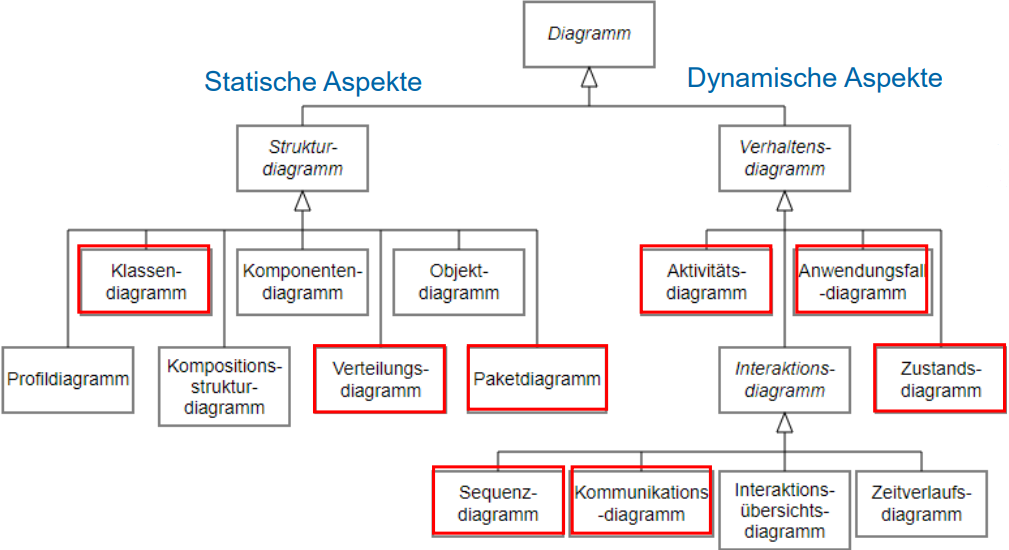
\includegraphics[width=0.3\textwidth]{Resources/Images/UML_Diagramme.png}
\caption{\label{fig:Guetereinteilung}Guetereinteilung.}
\end{figure}

\subsubsection{Gebrauch der UML}
\begin{itemize}
	\item UML as a sketch
	\begin{itemize}
		\item Informell, unvollständig
		\item Bevorzugt von agile Community
	\end{itemize}
	\item UML as blueprint
	\begin{itemize}
		\item Detallierte Analyse und Design-Diagramme für Code  
		\item Forward - und Reverse-Engineering
	\end{itemize}
	\item UML as a Programming Language
	\begin{itemize}
		\item Komplette, ausführbare Spezifikation eines Software-Systems in UML
		\item MDA-Tools zur Modellierung und Generierung
	\end{itemize}

\end{itemize}




















































\end{document}